\documentclass[times, utf8, zavrsni, numeric]{fer}
\usepackage{booktabs}
\usepackage{graphicx}
\usepackage{svg}
\usepackage{amsmath}
\usepackage{listings}
\usepackage[hidelinks]{hyperref}
\renewcommand{\vec}[1]{\mathbf{#1}}

\graphicspath{ {./images/} }

\begin{document}

% TODO: Navedite broj rada.
\thesisnumber{6346}

% TODO: Navedite naslov rada.
\title{Konvolucijski modeli za jednooku predikciju dubine scene}

% TODO: Navedite vaše ime i prezime.
\author{Filip Oreč}

\maketitle

% Ispis stranice s napomenom o umetanju izvornika rada. Uklonite naredbu \izvornik ako želite izbaciti tu stranicu.
\izvornik

% Dodavanje zahvale ili prazne stranice. Ako ne želite dodati zahvalu, naredbu ostavite radi prazne stranice.
\zahvala{Hvala}

\tableofcontents

\chapter{Uvod}
Predikcija dubine scene je još davno poznati problem. Konvencionalni
prikazi kao što su slika ili video prikazuju trodimenzionalni svijet u
dvije dimenzije. Naime, time gubimo informaciju o trećoj dimenziji koja
sadrži informaciju o dubini scene. Iako je dvodimenzionalna 
reprezentacija dovoljna u većini primjena, nekad nam je potrebna
trodimenzionalna reprezentacija. Percepcija dubine proizlazi iz
raznih znakova ili naznaka o dubini. Obično se dijele na binokularne 
znakove koji sadrže informacije u tri dimenzije i mogu se vidjeti s dva 
oka i monokularne znakove koji sadrže informacije u dvije dimenzije i 
mogu se vidjeti s jednim okom.\\\indent 
Tijekom godina razvile su se razne tehnike za predikciju dubine scene poput
stereoskopije koja se oslanja na binokularne znakove. Korištenjem dvije slike 
iste scene koje su dobivene iz malo drugačijih kuteva, moguće je izračunati 
udaljenost od objekta. Aplikacijama koje uključuju 
razumijevanje scene, 3D modeliranje i slično jako je bitna informacija o 
dubini kad gore navedena organizacija podataka i tehnike nisu dostupni.
U tom slučaju koristi se jednooka predikcija dubine scene koja predstavlja 
loše postavljen (engl. \textit{ill-posed}) problem, jer iz jedne dvodimenzionalne slike 
može nastati beskonačno mnogo različitih trodimenzionalnih scena. Za ljude 
ovo ne predstavlja veliki problem, jer možemo jako dobro iskoristiti 
monokularne znakove, ali za računala predstavlja ogroman problem za riješiti 
s velikom preciznosti i malom uporabom resursa.
Zbog navedenog razloga te jednostavnosti primjene, u zadnje vrijeme se sve
češće upotrebljavaju konvolucijske
neuronske mreže koji uče odnos između piksela boje i dubine, što je i predmet ovog
rada. Detaljnije ću obraditi konvolucijsku neuronsku mrežu predloženu u 
\cite{DBLP:journals/corr/LainaRBTN16}, te ju implementirati i primijeniti na
 problem jednooke predikcije dubine scene.\\\indent
U drugom poglavlju objašnjeni su osnovni pojmovi vezani uz umjetne neuronske
mreže, te osnovni algoritmi koji se koriste prilikom njihovog učenja. Treće
poglavlje opisuje konvolucijske neuronske mreže te zašto su one bitne. U sklopu
trećeg poglavlja još se opisuju rezidualne neuronske mreže i koje probleme
one rješavaju. Četvrto poglavlje bavi se detaljima implementacije predložene
arhitekture, te se ukratko opisuje korišteni programski okvir PyTorch.
U petom poglavlju su opisani rezultati koje je model ostvario.


\chapter{Umjetna neuronska mreža}

Nastanak umjetnih neuronskih mreža u početku je bio inspiriran biološkim 
neuronima i neuronskim mrežama, ali daljnjim razvojem su se odvojile od biološke
povezanosti i postale stvar inženjerstva. Definiraju se procesne jedinice 
zvane umjetni neuroni koji se međusobno povezuju te grade 
umjetne neuronske mreže. 
\\\indent Ovaj rad se bavi samo unaprijednim neuronskim
mrežama (engl. \textit{feedforward neural networks}). Cilj unaprijedne
neuronske mreže je aproksimirati neku funkciju $f^*$, tako da definira
preslikavanje $\vec{y} = f(\vec{x};\pmb{\theta})$ i nauči vrijednost
parametara $\pmb{\theta}$ kako bi najbolje aproksimirala ciljanu funkciju $f^*$.
Ovakvi modeli zovu se unaprijedni jer nema veza koje izlaze iz modela vraćaju
nazad na ulaze.


\section{Umjetni neuron}
Warren McCulloch i Walter Pitts 1943. godine konstruirali su matematički model
neurona kakav je prikazan na slici \ref{fig:umjetni_neuron}.

\begin{figure}[htbp]
	\centering
	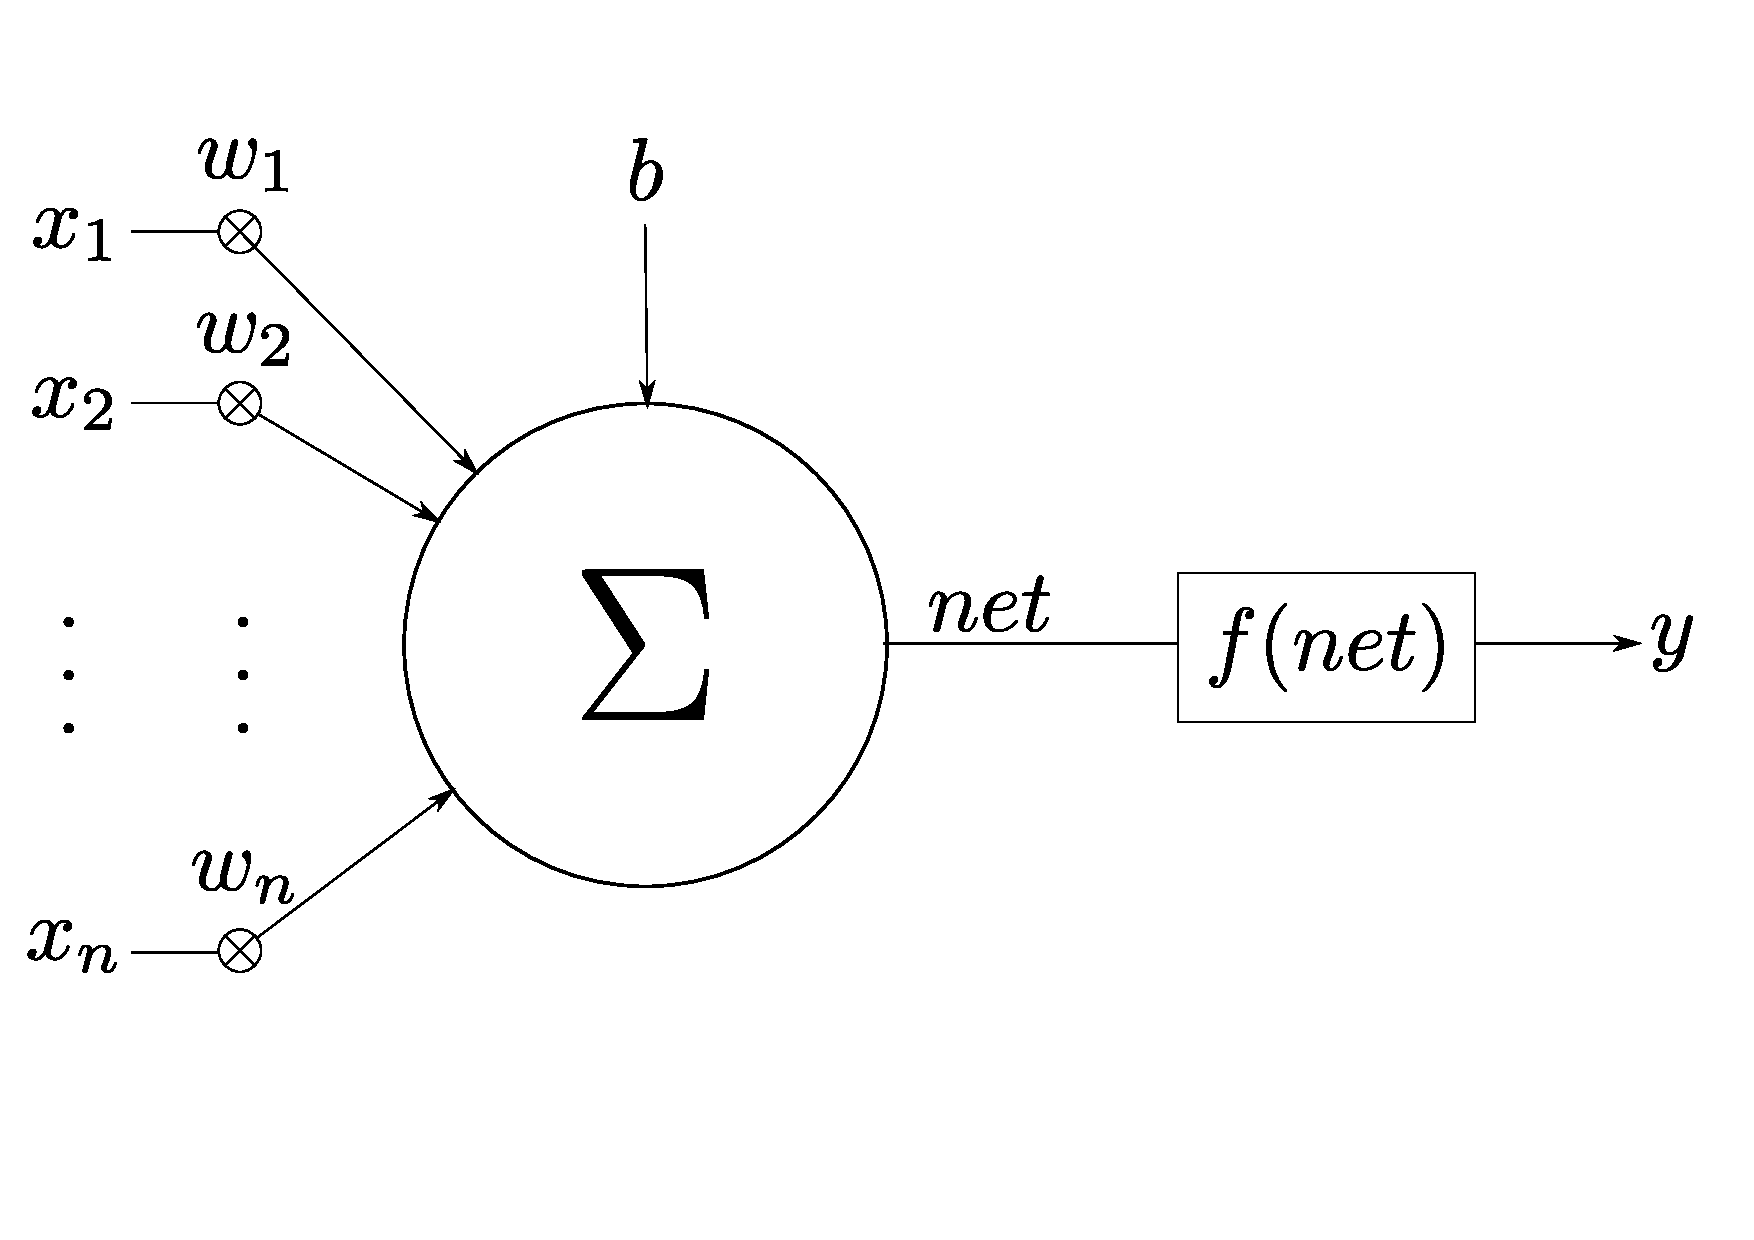
\includegraphics[scale=0.3]{moj_umjetni_neuron.pdf}
	\caption{Umjetni neuron}
	\label{fig:umjetni_neuron}
\end{figure}

Umjetni neuron prima više ulaza $x_1, x_2,...,x_n$ koji tvore ulazni 
vektor $\vec{x}$. Taj ulazni vektor može biti stvarni ulaz ili izlaz iz nekog 
prethodnog neurona. Za svaku vrijednost $x_i$ ulaznog vektora $\vec{x}$
postoji vrijednost $w_i$ koju nazivamo težina (eng. \textit{weight}). To je 
vrijednost koja predstavlja utjecaj ulaza $x_i$ na neuron. Svaki ulaz $x_i$ 
množi se s odgovarajućom težinom $w_i$ što daje umnožak $x_i \cdot w_i$. 
Vrijednosti $w_1, w_2,...,w_n$ tvore vektor težina $\vec{w}$. Još se definira
i vrijednost $b$ koja označava pomak (engl. \textit{bias}). Sve primljene 
vrijednosti se sumiraju prema izrazu \ref{eq: net}.
\begin{equation}
	net = \sum_{i=1}^{n}x_i \cdot w_i + b
	\label{eq: net}
\end{equation}
Izraz \ref{eq: net} može se zapisati u matričnom obliku:
\begin{equation}
	net = \vec{w}^\top \cdot \vec{x} + b
\end{equation}
Pri tome ulazni vektor $\vec{x}$ i vektor težina $\vec{w}$ imaju dimenzije 
N$\times$1, gdje N predstavlja broj ulaza u neuron, dok je pomak $b$ skalar.
Rezultat sumiranja $net$ dalje se predaje kao ulaz prijenosnoj funkciji koja
određuje konačni izlaz $o$ neurona prema izrazu \ref{eq: output}.
\begin{equation}
	y = f(net) = f(\vec{w}^\top \cdot \vec{x} + b)
	\label{eq: output}
\end{equation}
Gdje $f$ predstavlja prijenosnu funkciju.

\subsection{Prijenosne funkcije}
Glavna zadaća prijenosne funkcije je pretvorba ulaznih vrijednosti u izlaznu 
vrijednost. Pri tome se mogu koristiti različite vrste funkcija ovisno o 
arhitekturi mreže. Danas postoji više prijenosnih funkcija koje se češće koriste.
\\\indent
Prva od njih je funkcija skoka i definirana je izrazom \ref{eq:step_fun}.
\begin{equation}
	u(x) = 
	\begin{cases}
		0, \quad x < 0\\
		1, \quad x \geq 0
	\end{cases}
	\label{eq:step_fun}
\end{equation}

Bitno svojstvo ove funkcije je prekid u točki $x=0$, te zbog toga nije 
diferencijabilna u toj točki. Naime, to svojstvo onemogućava korištenje 
algoritama učenja koji se temelje na gradijentu. 
\begin{figure}[htb]
	\centering
	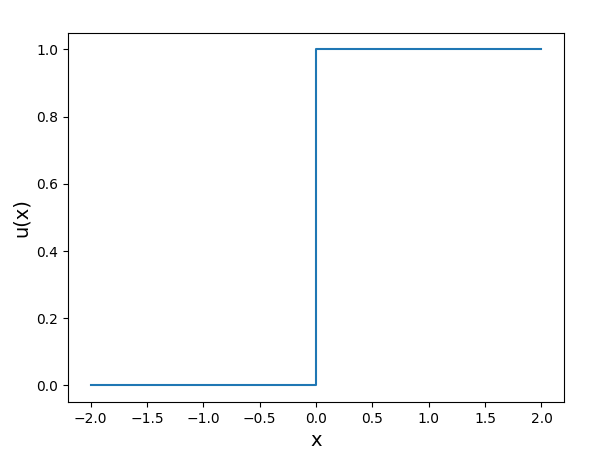
\includegraphics[scale=0.35]{step_fun.png}
	\caption{Funkcija skoka}
	\label{fig:step_fun}
\end{figure}
Izgled funkcije prikazan je na slici 
\ref{fig:step_fun}.
\newpage
Sigmoidalna funkcija ima jako dobra svojstva te se zbog toga često primjenjuje.
Smješta bilo koji realni broj na interval $[0, 1]$. Definirana je izrazom 
\ref{eq:sig}.
\begin{equation}
	\sigma(x)=\frac{1}{1+e^{-x}}
	\label{eq:sig}
\end{equation}
Ova funkcija ima dosta sličnosti s funkcijom skoka. Naime, ako je $x$ neki 
veliki pozitivan broj onda je $e^{-x} \approx 0$, i izlaz iz neurona je blizu
1. S druge strane ako je $x$ neki veliki negativni broj onda $e^{-x} \to 
\infty$, i izlaz iz neurona je blizu 0. To se jako dobro može primijetiti na
grafu funkcije prikazanom na slici \ref{fig:sig_fun}.
\begin{figure}[htb]
	\centering
	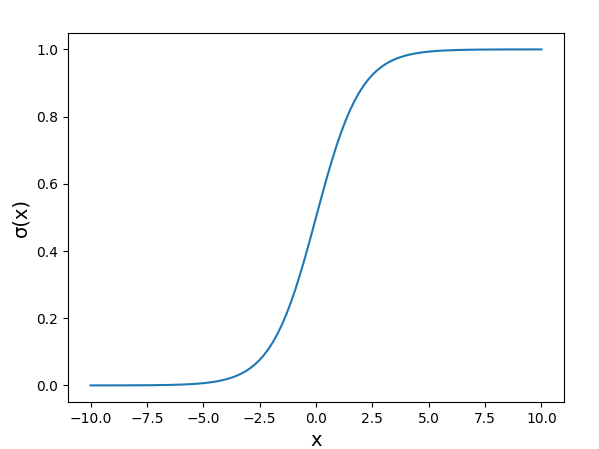
\includegraphics[scale=0.35]{sig_fun.png}
	\caption{Sigmoidalna funkcija}
	\label{fig:sig_fun}
\end{figure}

Velika prednost sigmoidalne funkcije u odnosu na funkciju skoka je činjenica da 
je derivabilna, što omogućava korištenje algoritama učenja koji se temelje na 
gradijentu. Derivacija ove funkcije dana je izrazom \ref{eq:dsig}.
\begin{equation}
	\frac{d\sigma(x)}{dx} = \sigma(x)\cdot(1-\sigma(x))
	\label{eq:dsig}
\end{equation}

Na krajevima funkcija jako slabo reagira na promjene i zato će gradijent u tim 
dijelovima imati male vrijednosti. Ako mreža uči pomoću lokalnih gradijenata,
u tom slučaju učenje staje, jer gradijenti ne mogu napraviti značajne promjene.
\\\indent
Funkciju tangens hiperbolni moguće je dobiti izravno iz sigmoidalne funkcije.
Definicija je dana izrazom \ref{eq:tanh}.
\begin{equation}
	tanh(x) = 2\sigma(2x)-1
	\label{eq:tanh}
\end{equation}
Ova prijenosna funkcija smješta bilo koji realni broj na interval $[-1, 1]$.
Prednost je što je derivabilna, ali kao i sigmoidalna funkcija na krajevima jako
slabo reagira na promjene, te ako je vrijednost ulaza u funkciju u tom području, 
učenje staje, što se može vidjeti na grafu funkcije \ref{fig:tanh_fun}. Derivacija 
funkcije dana je izrazom \ref{eq:dtanh}.
\begin{equation}
	\frac{dtanh(x)}{dx} = 1 - tanh^2(x)
	\label{eq:dtanh}
\end{equation}
\begin{figure}[htb]
	\centering
	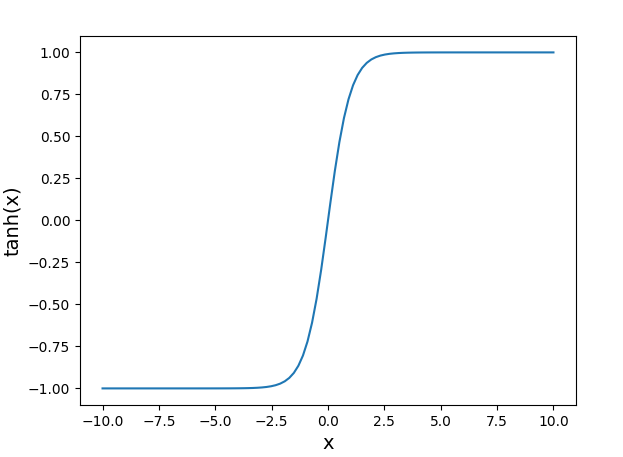
\includegraphics[scale=0.35]{tanh_fun.png}
	\caption{Tangens hiperbolni}
	\label{fig:tanh_fun}
\end{figure}

Zadnjih nekoliko godina sve se češće koristi ReLU (\textit{Recitified Linear 
Unit}) prijenosna funkcija. Određena je izrazom \ref{eg:relu}.
\begin{equation}
	relu(x) = max(0, x)
	\label{eg:relu}
\end{equation}
Ova prijenosna funkcija sve vrijednosti veće od 0 propušta, dok vrijednosti manje 
od 0 uopće ne propušta, što se može vidjeti na grafu funkcije \ref{eg:relu}.
\begin{figure}[htb]
	\centering
	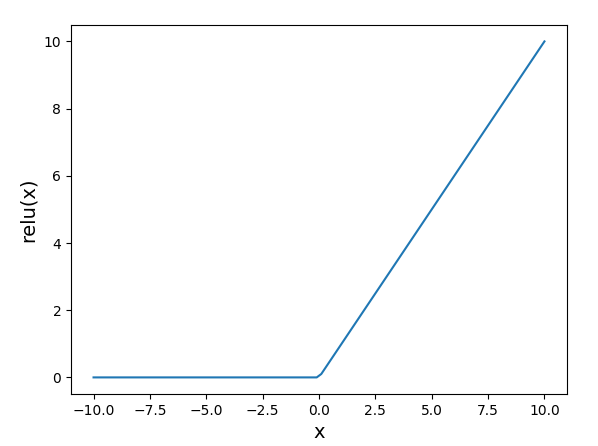
\includegraphics[scale=0.35]{relu_fun.png}
	\caption{ReLU}
	\label{fig:relu_fun}
\end{figure}
\\
Derivacije ove funkcije dana je izrazom \ref{eq:drelu}.
\begin{equation}
	\frac{drelu(x)}{dx} = 
	\begin{cases}
		1, \quad x > 0\\
		0, \quad x \leq 0
	\end{cases}
	\label{eq:drelu}
\end{equation}
Razlog zbog kojeg se sve češće primjenjuje je brzina računanja. Ali i ova 
prijenosna funkcija ima nedostatak. Iz izraza \ref{eq:drelu} se vidi da je 
za sve negativne brojeve derivacija jednaka 0, što predstavlja problem za
algoritme učenja temeljene na gradijentu. Neuron kojemu je suma ulaza, odnosno
$net$ negativan, se zbog toga neće moći prilagođavati.

\section{Arhitektura umjetne neuronske mreže}
Umjetna neuronska mreža sastoji se od više umjetnih neurona koji su međusobno
povezani i grupirani u slojeve. Na slici \ref{fig:ann} je prikazana neuronska
mreža koja ima četiri sloja. Prvi sloj je ulazni i sastoji se od tri neurona,
a zadnji sloj je izlazni i sastoji se od dva neurona. Svaki sloj koji se nalazi
između ulaznog i izlaznog zove se skriveni sloj. 

\begin{figure}[htb]
	\centering
	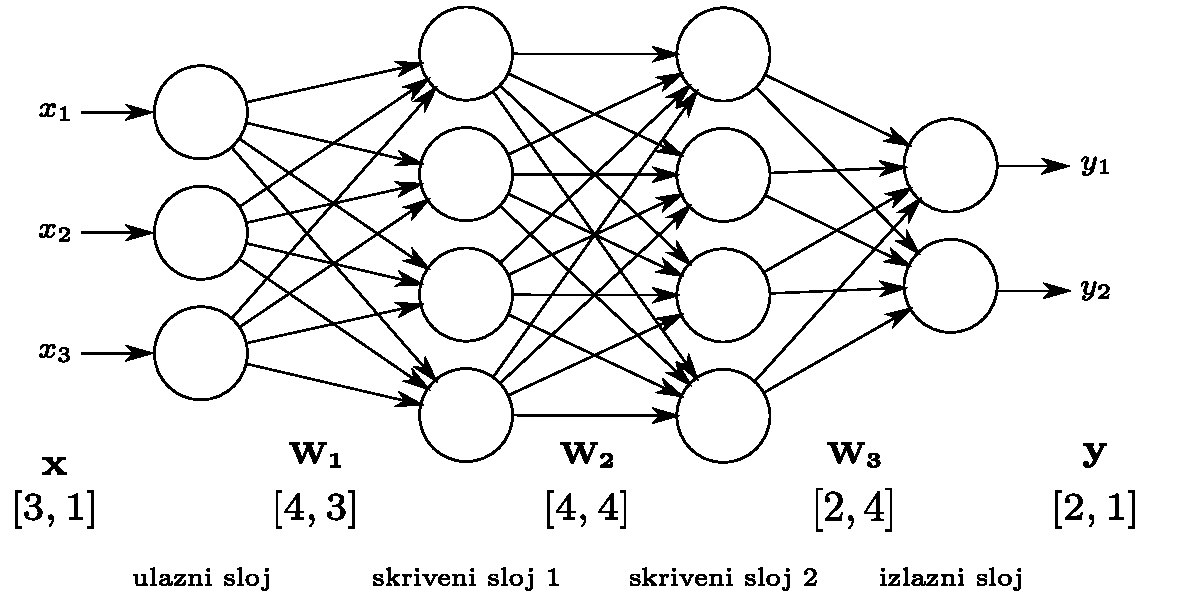
\includegraphics[scale=0.65]{ann.pdf}
	\caption{Umjetna neuronska mreža}
	\label{fig:ann}
\end{figure}

Ovakva mreža zove se još i 
potpuno povezana mreža, jer je izlaz iz svakog neurona u jednom sloju povezan 
sa svim neuronima u idućem sloju. Arhitektura neuronske mreže opisuje
kompoziciju funkcija. Na primjer, mrežu sa slike \ref{fig:ann} možemo opisati 
kompozicijom funkcija $f(\vec{x}) = f^{(3)}(f^{(2)}(f^{(1)}(\vec{x})))$, gdje
$f^{(1)}$ predstavlja prvi skriveni sloj, $f^{(2)}$ drugi skriveni sloj, a
$f^{(3)}$ izlazni sloj. Pri tome su funkcije $f^{(1)}$, $f^{(2)}$, $f^{(3)}$
definirane izrazima: 
\begin{align}
	\vec{h_1} &= f^{(1)}(\vec{x};\vec{W_1}, \vec{b_1}) = g_1(\vec{W_1}\cdot
	\vec{x} +\vec{b_1}) \\
	\vec{h_2} &= f^{(2)}(\vec{h_1};\vec{W_2}, \vec{b_2})= g_2(\vec{W_2}\cdot
	\vec{h_1} +\vec{b_2}) \\
	\vec{y} &= f^{(3)}(\vec{h_2};\vec{W_3}, \vec{b_3}) = g_3(\vec{W_3}\cdot
	\vec{h_2} +\vec{b_3})
\end{align}

Gdje $g_1$, $g_2$ i $g_3$ predstavljaju prijenosne funkcije u pojedinim 
slojevima, a matrice $\vec{W_1}$, $\vec{W_2}$ i $\vec{W_3}$ predstavljaju
matrice težina pojedinih slojeva. Vektori $\vec{b_1}$, $\vec{b_2}$ i $\vec{b_3}$
predstavljaju pomak za svaki sloj.

\section{Učenje umjetne neuronske mreže}
Učenje neuronske mreže je proces nalaženja optimalnih parametara $\pmb{\theta}$,
kako bi neuronska mreža što bolje aproksimirala ciljnu funkciju. Ciljna funkcija
se zaključuje na osnovu uzoraka iz skupa za učenje koji se predočavaju 
neuronskoj mreži. Svaki uzorak je par koji se sastoji od ulaza u mrežu i
željenog izlaza. Ovakav način učenja se zove nadzirano učenje (engl. 
\textit{supervised learning}).
\\\indent
Kako bi odredili koliko dobro mreža aproksimira ciljnu funkciju koristimo
funkciju gubitka. Optimiziranjem funkcije gubitka neuronska mreža se uči.

\subsection{Funkcija gubitka}
Kako bi se moglo ostvariti učenje, potrebno je definirati funkciju gubitka,
koja ovisi o parametrima $\pmb{\theta}$, tj. o težinama $\vec{W}$ i pomacima
$\vec{b}$. Kao i prijenosna funkcija, funkcija gubitka se može definirati
na više načina.
\\\indent Najčešće funkcije gubitka za regresijske probleme su $\mathcal{L}_1$ i
$\mathcal{L}_2$ funkcije gubitka. Definirane su sljedećim izrazima:
\begin{align}
	\mathcal{L}_1 &= \sum_{i=0}^{n}|y_i - \hat{y_i}| \\
	\mathcal{L}_2 &= \sum_{i=0}^{n}(y_i - \hat{y_i})^2
\end{align}
gdje $y_i$ predstavlja ispravnu vrijednost, $\hat{y_i}=f(\vec{x})$ procijenjenu 
vrijednost, a $n$ broj podataka. 
\\\indent Za probleme klasifikacije se $\mathcal{L}_1$ i $\mathcal{L}_2$ 
funkcije gubitka ne koriste toliko često.
Za ovaj problem se pretežito koristi unakrsna entropija (engl. \textit{cross-
entropy loss}). Definirana je izrazom \ref{eq:cross}.
\begin{equation}
	\mathcal{L}_{CE} = -\sum_{i=0}^n y_i \cdot log(\hat{y_i})
	\label{eq:cross}
\end{equation}

\subsection{Gradijentni spust}
Optimiziranjem funkcije gubitka parametri neuronske mreže se "štimaju" i mreža 
uči. Za optimiziranje funkcije gubitka koristi se gradijentni spust.
To je iterativni optimizacijski algoritam za pronalaženje minimuma funkcije.
\\\indent Ako je funkcija $y = f({x})$, gdje su $x$ i $y$ realni brojevi, 
funkcija koja se optimizira, onda je derivacija te funkcije 
$f'(x) = \frac{dy}{dx}$. Tada je aproksimacija funkcije $f(x)$ Taylorovim 
razvojem prvog reda:
\begin{equation}
	f(x+\Delta x) \approx f(x) + f'(x)\cdot \Delta x
\end{equation}
Ako se u tu aproksimaciju uvrsti pomak u smjeru gdje funkcija pada, odnosno u
smjeru negativne derivacije dobiva se:
\begin{equation}
	f(x -\epsilon \cdot sign(f'(x))) \approx f(x) - f'(x)\cdot\epsilon \cdot 
	sign(f'(x))
\end{equation}
Vidi se da je $f(x -\epsilon \cdot sign(f'(x)))$ manje od $f(x)$ za dovoljno
mali $\epsilon$. Dakle, ako se $x$ iterativno pomiče malim koracima sa
suprotnim predznakom derivacije, može se doći do minimuma funkcije.
\\\indent Za funkcije više varijabli koriste se parcijalne derivacije i 
gradijent funkcije. Parcijalna derivacija $\frac{\partial}{\partial x_i}
f(\vec{x})$ određuje koliko se $f$ promijeni ako se jedino $x_i$ poveća u 
točki $\vec{x}$. Gradijent funkcije $\nabla f(\vec{x})$ je vektor koji 
sadrži sve parcijalne derivacije funkcije. Dan je izrazom \ref{eq:grad}.
\begin{equation}
	\nabla f(\vec{x}) = \bigg[\frac{\partial f}{\partial x_1},
	\frac{\partial f}{\partial x_2}, \cdots ,
	\frac{\partial f}{\partial x_n}\bigg]
	\label{eq:grad}
\end{equation}
Aproksimacija funkcije više varijabli Taylorovim razvojem prvog reda je dana
sljedećim izrazom:
\begin{equation}
	f(\vec{x} + \Delta \vec{x}) \approx f(\vec{x}) + \nabla f(\vec{x})^\top
	\Delta \vec{x}
\end{equation}
Ako se u danu aproksimaciju uvrsti pomak u smjeru najbržeg pada funkcije, 
odnosno u smjeru negativnog gradijenta funkcije dobiva se:
\begin{equation}
	f(\vec{x} - \epsilon \cdot \nabla f(\vec{x})) \approx f(\vec{x}) - \epsilon
	\cdot \nabla f(\vec{x})^\top \nabla f(\vec{x})
\end{equation}
gdje $\epsilon$ predstavlja mali pozitivan parametar koji se češće zove
korak učenja. Kako je $\nabla f(\vec{x})^\top \nabla f(\vec{x}) \geq 0$,
funkcija $f(\vec{x})$ će se smanjivati sve dok ne dođe do minimuma gdje je
$\nabla f(\vec{x}) = \vec{0}$. Za sljedeću iteraciju $\vec{x}$ se ažurira 
izrazom \ref{eq:x_upd} i postupak se ponavlja za točku $\vec{x}'$.
\begin{equation}
	\vec{x}' = \vec{x} - \epsilon\cdot \nabla f(\vec{x})
	\label{eq:x_upd}
\end{equation}
\indent Ako funkcija $f$ predstavlja funkciju gubitka $\mathcal{L}$ 
onda se svakim korakom
gradijentnog spusta ažuriraju se parametri neuronske mreže izrazima:
\begin{align}
	\vec{w}' &= \vec{w} - \epsilon \cdot \nabla_\vec{w} \mathcal{L}(\vec{w}, 
	\vec{b}) \\
	\vec{b}' &= \vec{b} - \epsilon \cdot \nabla_\vec{b} \mathcal{L}(\vec{w}, 
	\vec{b})
\end{align}
\indent Ako je skup podatak za učenje velik, računanje gradijenta za sve podatke
odjednom može biti sporo. Postupak se može ubrzati korištenjem stohastičkog
gradijentnog spusta. Korak gradijentnog spusta se računa samo za dio skupa za 
učenje (engl. \textit{batch}). Prolazak kroz cijeli skup za učenje naziva se 
epoha. Ovaj način također omogućava i bolje izbjegavanje lokalnih minimuma.

\subsection{Optimizacija}
Učenje neuronske mreže gradijentnim spustom može se ubrzati raznim 
optimizacijskim metodama. 
\\\indent Jedna od tih metoda je momentum. Definira se novi vektor $\vec{v}$,
te se mijenja jednadžba za ažuriranje parametara gradijentnog spusta
na sljedeći način:
\begin{equation}
\begin{aligned}
	\vec{v}' &= \alpha \vec{v} - \epsilon \nabla \mathcal{L} \\
	\vec{w}' &= \vec{w} + \vec{v}'
\end{aligned}
\end{equation}
gdje je $\alpha \in [0, 1)$ hiperparametar koji modelira prigušenje koje
omogućuje zaustavljanje u minimumu. Najčešće se inicijalizira na $0.9$. 
Vektor $\vec{v}$ predstavlja brzinu kretanja prema minimumu, što je gradijent
veći, brzina će se sve više povećavati.

\subsection{Regularizacija}
Neuronska mreža mora imati dobre rezultate izvođenja ne samo na skupu 
podataka za učenje, nego i na novim podatcima. Razvijene su razne metode
kako bi se smanjila pogreška na novim podatcima, pa čak i ako se poveća
pogreška na skupu za učenje. Ove metode poznate su kao regularizacija.
\\\indent Jedna od metoda je dodavanje funkciji gubitka dodatni član:
\begin{equation}
	\mathcal{L}_r = \mathcal{L} + \lambda N(w)
\end{equation}
gdje je $\mathcal{L}$ gubitak, a $\lambda$ je hiperparametar koji određuje
utjecaj regularizacijskog člana. Ako regularizacijski član odgovara
$L^1$-normi ili $L^2$-normi, onda se ova metoda zove $L^1$-regularizacija, 
odnosno $L^2$-regularizacija. U tom slučaju funkcija gubitka se može ovako
napisati:
\begin{align}
	\label{eq:l1_reg}
	\mathcal{L}_r &= \mathcal{L} + \lambda \sum_i |w_i|	 \\
	\mathcal{L}_r &= \mathcal{L} + \lambda \sum_i w_i^2
	\label{eq:l2_reg}
\end{align}
gdje se jednadžba \ref{eq:l1_reg} odnosi na $L^1$-regularizaciju, a 
\ref{eq:l2_reg} na $L^2$ regularizaciju. Posljedica dodavanja regularizacijskog
člana je preferiranje učenja manjih težina.
\\\indent Sljedeća metoda je dropout, koja se dosta razlikuje od $L^1$ i 
$L^2$ regularizacije. Ova metoda se ne oslanja na izmjenjivanje funkcije 
gubitka nego na izmjenjivanje same mreže. Svaki neuron u skrivenom sloju
s određenom vjerojatnošću privremeno postaje isključen tijekom učenja.
Tako se sprječava da utjecaj nekih neurona postane prevelik i tako uzrokuje prenaučenost.
\\\indent Povećavanje skupa za učenje je još jedan način kako smanjiti
prenaučenost. Dobivanje novih podataka za učenje može biti skupo i nije
uvijek moguće. Zato se postojeći skup podataka za učenje može proširiti
raznim transformacijama. To mogu biti razne transformacije poput rotacije,
zrcaljenja, skaliranja, izmjene svjetline i kontrasta. 
\\\indent Još jedan oblik regularizacije je normalizacija nad grupama
(engl. \textit{batch-normalization}). Izlaz iz svakog sloja se normalizira. 
Ako je $\mu_B$ aritmetička sredina, a $\sigma_B^2$ varijanca podataka mini grupe $B$, tada za sloj s ulazom $x = (x^{(1)}, ..., x^{(d)})$ se primjenjuje 
normalizacija:
\begin{equation}
	\hat{x}^{(k)} = \frac{x^{(k)} - \mu_B}{\sqrt{\sigma_B^2 + \epsilon }}
\end{equation}
Bez normalizacije male promjene u prvim slojevima će se povećati kako se 
propagiraju kroz mrežu, što rezultira velikim promjenama u dubljim slojevima.
Metoda normalizacije nad grupama smanjiva ovakve neželjene promjene i tako
ubrzava proces treniranja. Kako ova metoda koristi srednju vrijednost i 
varijancu grupe koje su svaku epohu različite, model ne trenira na istim
podatcima i tako se postiže regularizacija.

\subsection{Propagacija pogreške unatrag}
Propagacija pogreške unatrag (engl. \textit{back-propagation}) je algoritam
za učinkovito računanje gradijenata funkcije putem rekurzivne primjene pravila
ulančavanja. Dakle, za neku funkciju $f(\vec{x})$ gdje je $\vec{x}$ ulazni vektor,
algoritam propagacije pogreške unatrag računa gradijent funkcije $f$ u 
točki $\vec{x}$, tj. $\nabla f(\vec{x})$. Za slučaj učenja neuronske mreže
gradijentnim spustom, funkcija $f$ će odgovarati funkciji gubitka $\mathcal{L}$
, a ulazni
vektor $\vec{x}$ će se sastojati od podataka za učenje, težina $\vec{W}$ i 
pomaka $\vec{b}$ neuronske mreže. 
\\\indent U konačnici, to znači računanje parcijalnih derivacija
$\partial \mathcal{L} / \partial w_{jk}^l$ i $\partial \mathcal{L} / \partial b_{j}^l$, gdje $w_{jk}^l$ označava težinu koja povezuje $k$-ti neuron u $(l-1)$-om
sloju s $j$-tim neuronom u $l$-tom sloju. Slično, $b_{j}^l$ označava pomak
$j$-tog neurona u $l$-tom sloju. Za računanje ovih parcijalnih derivacija
uvodi se pogreška $\delta_j^l$ neurona $j$ u sloju $l$:
\begin{equation}
	\delta_j^l = \frac{\partial \mathcal{L}}{\partial net_j^l}
\end{equation}
gdje $net_j^l$ predstavlja izlaz iz neurona prije primjene aktivacijske funkcije
definiran jednadžbom \ref{eq: net}. Za pogrešku neurona $\delta_j^L$
u izlaznom sloju vrijedi:
\begin{equation}
	\delta_j^L = \frac{\partial \mathcal{L}}{\partial y_j^L}
	\frac{\partial y_j^L}{\partial net_j^L} = 
	\frac{\partial \mathcal{L}}{\partial y_j^L} f'(net_j^L)
	\label{eq:neuron_err}
\end{equation}
gdje $y_j^L$ predstavlja izlaz iz neurona, a $f$ prijenosnu funkciju definirane
jednadžbom \ref{eq: output}. Jednadžba \ref{eq:neuron_err} može se zapisati
u matričnom obliku:
\begin{equation}
	\delta^L = \nabla_{y} \mathcal{L} \odot f'(net^L)
	\label{eq:neuron_err_mat}
\end{equation}
gdje $\odot$ predstavlja umnožak matrica gdje se elementi na istim mjestima
množe. Primjenom ove jednadžbe mogu se dobiti pogreške samo za neurone
izlaznog sloja, ali poznavanjem pogrešaka nekog sloja mogu se dobiti 
pogreške prethodnog sloja. Pogreške skrivenih slojeva se izračunavaju
prema izrazu:
\begin{equation}
	\delta^l = ((w^{l+1})^\top \delta^{l+1}) \odot f'(net^l)
	\label{eq:hid_neuron_err_mat}
\end{equation}
Jednadžbama \ref{eq:neuron_err_mat} i \ref{eq:hid_neuron_err_mat} može se
izračunati pogreška $\delta^l$ za svaki sloj mreže. Prvo se izračuna
pogreška izlaznog sloja $\delta^L$ pomoću jednadžbe \ref{eq:neuron_err_mat},
zatim se pomoću jednadžbe \ref{eq:hid_neuron_err_mat} izračuna pogreška
$\delta^{L-1}$, zatim pogreška $\delta^{L-2}$ i sve tako do ulaznog sloja
mreže.\\\indent
Parcijalna derivacija s obzirom na pomak odgovara upravo pogrešci neurona:
\begin{equation}
	\frac{\partial \mathcal{L}}{\partial b_j^l} = \delta_j^l
	\label{eq:dL_db}
\end{equation}
dok je parcijalna derivacija s obzirom na težinu neurona:
\begin{equation}
	\frac{\partial \mathcal{L}}{\partial w_{jk}^l} = y_k^{l-1} \delta_j^l
	\label{eq:dL_dw}
\end{equation}
Jednadžbama \ref{eq:dL_db} i \ref{eq:dL_dw} izračunava se ovisnost funkcije
gubitka o
pojedinim parametrima, što je i cilj algoritma propagacije pogreške unatrag.

\chapter{Konvolucijska neuronska mreža}
Konvolucijske neuronske mreže (engl. \textit{convolutional neural networks}) 
su posebna vrsta neuronskih mreža za obradu podataka koji imaju rešetkastu
(engl. \textit{grid-like}) topologiju. Najbolji primjer su slikovni podatci,
koji se mogu smatrati kao 2D rešetka piksela. 
\\\indent Kod tradicionalnih potpuno povezanih neuronskih mreža izlaz iz
svakog neurona u jednom sloju je povezan sa svakim neuronom u sljedećem sloju.
Za slike dimenzija HxWxC ulaz u mrežu je dimenzija $H \cdot W \cdot C$ što
znači da će samo jedan neuron u prvom skrivenom sloju
imati $H \cdot W \cdot C$ težina. Neuronska mreža u većini slučajeva ima
više od jednog neurona u skrivenom sloju te će doći do pojave previše
parametara.
\\\indent Konvolucijske neuronske mreže imaju prorijeđenu interakciju između
neurona, što znači da je potrebno pohraniti manje parametara i da izračunavanje 
izlaza zahtjeva manje operacija. Na slici \ref{fig:pror} je označen neuron
$x_3$ i izlazni neuroni $\vec{s}$ koji su povezani s tim neuronom. Lijevo
je prikazana prorijeđena interakcija, a desno potpuno povezana.
\begin{figure}[htb]
	\centering
	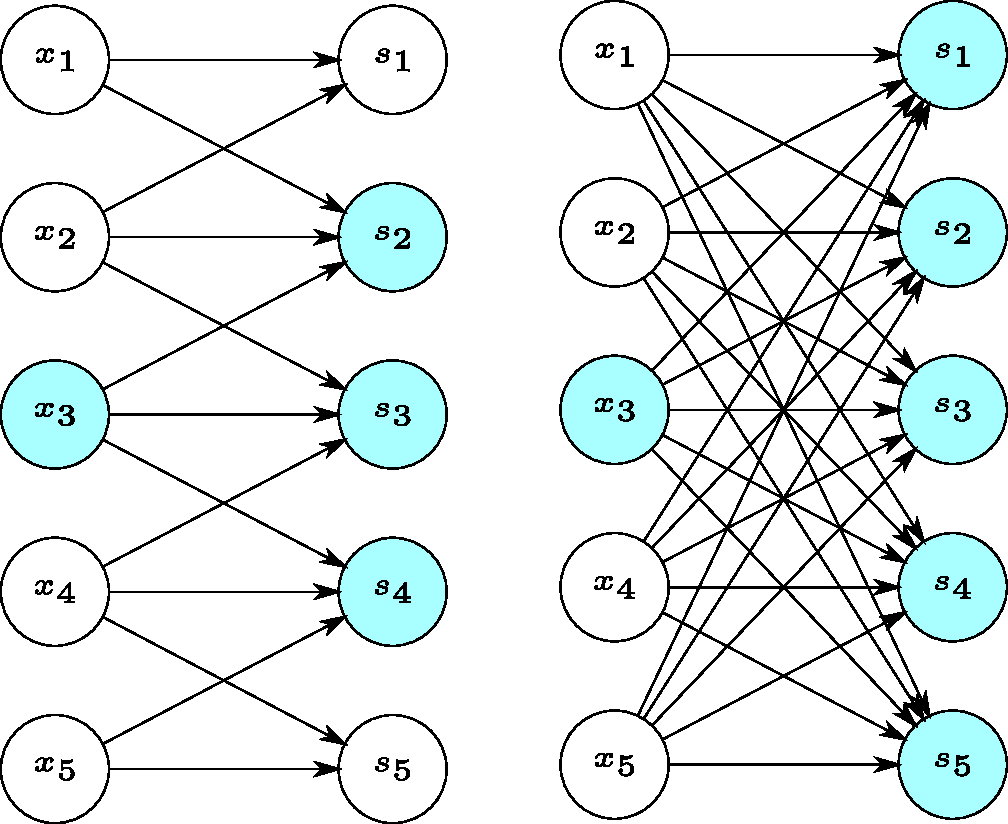
\includegraphics[scale=0.45]{pror.pdf}
	\caption{Primjer prorijeđene interakcije neurona}
	\label{fig:pror}
\end{figure}
\\\indent Slojevi konvolucijske neuronske mreže su organizirani u tri 
dimenzije: visina, dužina i dubina. Neuroni u pojedinom sloju su povezani
samo s malim dijelom neurona u prethodnom sloju, a ne sa svim neuronima kao
kod potpuno povezanih slojeva. Konvolucijske neuronske mreže grade se od
tri osnovna sloja: konvolucijski sloj, sloj sažimanja i potpuno povezani sloj.
\\\indent \textbf{Konvolucijski sloj} je temeljni sloj konvolucijske 
neuronske mreže. Parametri ovog sloja sastoje se od skupa filtera koji
se mogu naučiti. Filteri su prostorno dosta manjih dimenzija od ulaza u 
sloj. Izlazi se izračunavaju tako da se primjenjuje dvodimenzionalna
konvolucija ulaza s filterom čime se dobiva dvodimenzijska mapa
značajki. Na slici \ref{fig:conv} filter je dimenzija 2x2, dok je ulaz
dimenzija 3x4. Filter se pomjera po dužini i visini ulaza i izračunava se
skalarni produkt između članova filtera s članovima ulaza na odgovarajućim
pozicijama. Na kraju se dobiva mapa značajki s dimenzijama 2x3.
\begin{figure}[htb]
	\centering
	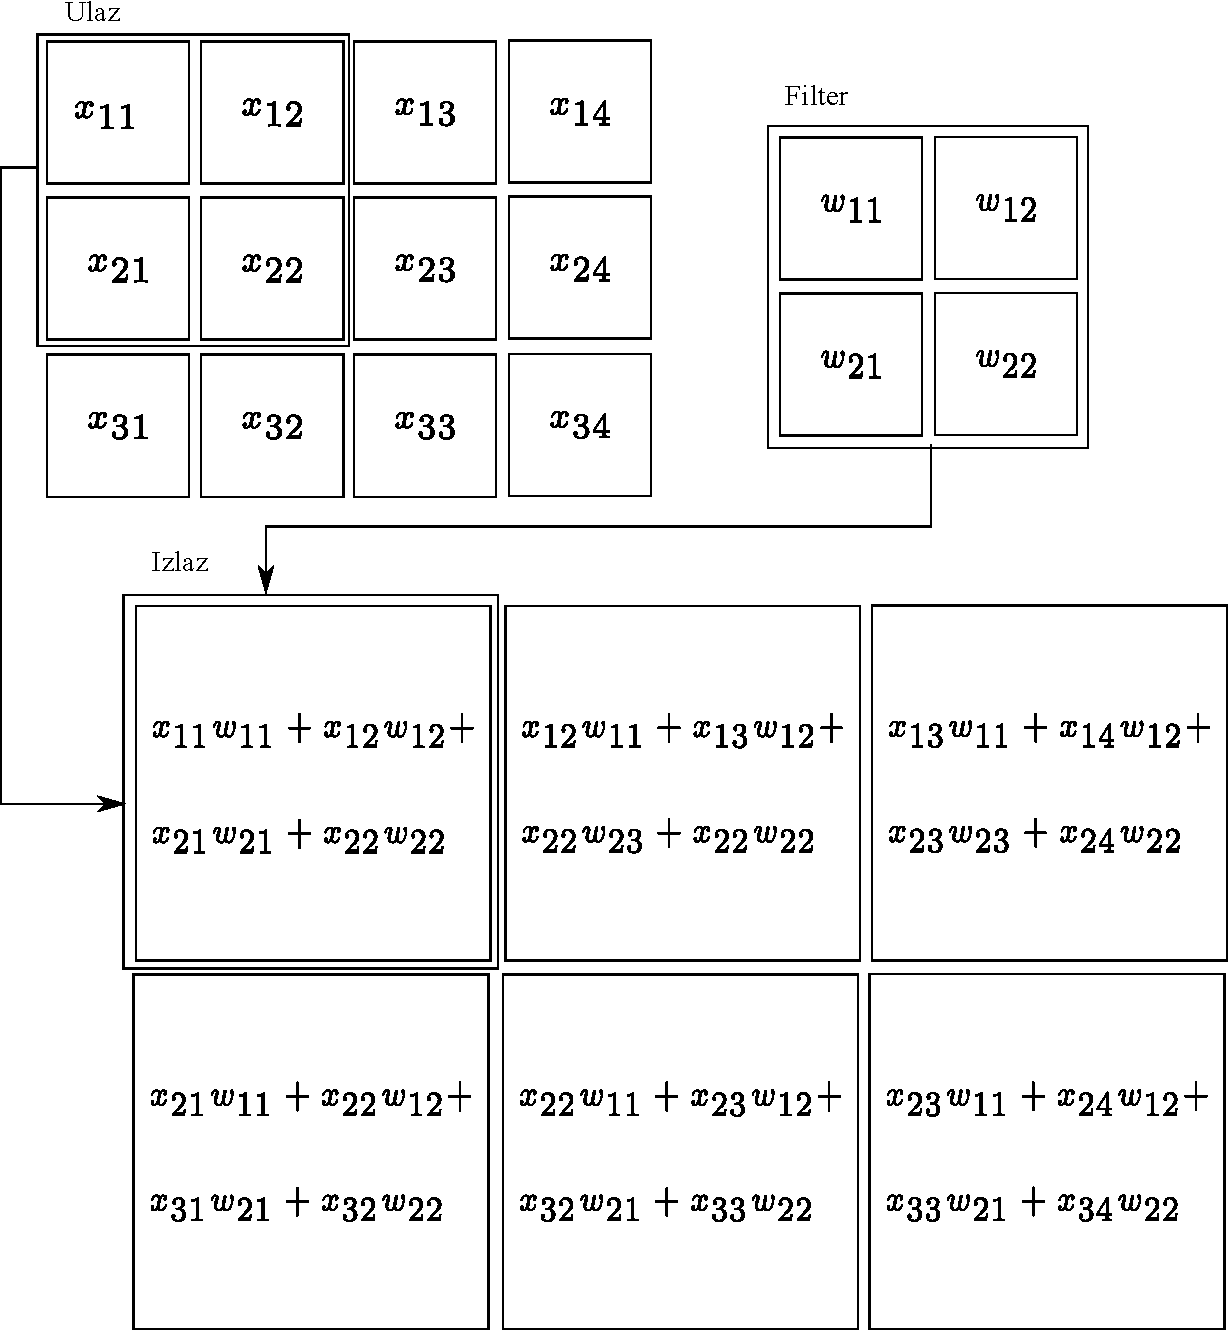
\includegraphics[scale=0.40]{conv.pdf}
	\caption{Konvolucija ulaza i filtera}
	\label{fig:conv}
\end{figure}
Konvolucijski slojevi obično imaju više filtera, i svaki od njih će 
izračunati zasebnu mapu značajki koje se slažu po dubini i tako stvaraju
izlaz. Na dobivene izlaze još se primjenjuje prijenosna funkcija. Broj
neurona koji su povezani s neuronom u sljedećem sloju
zove se receptivno polje neurona i odgovara upravo veličini filtera.
\\\indent Kako bi izlazne mape značajki imale istu visinu i dužinu kao i ulaz
ponekad je potrebno nadopuniti ulaz kako filter prilikom konvolucije ne bi
prelazio rubove ulaza. Najčešće se koristi nadopunjavanje nulama. Filter
se ne mora uvijek micati samo po jedan neurona, ali ako se miće po više 
neurona odjednom dimenzija izlaza će se smanjiti. Broj za koji se filter
miće zove se korak (engl. \textit{stride}).
\\\indent \textbf{Sloj sažimanja} je sloj koji smanjiva prostorne dimenzije 
(visinu i dužinu) ulaza kako bi se smanjio broj parametara neuronske mreže.
Primjenjuje se nezavisno na svakoj od mapi značajki. Sažimanje se može
ostvariti na više načina, ali se najčešće koristi sažimanje maksimalnom 
vrijednošću (engl. \textit{max-pooling}). Odabire se veličina i korak filtera,
te se primjenjuje funkcija sažimanja na područje koje odgovara trenutnoj
poziciji filtera. Na slici \ref{fig:max_pool} je prikazano sažimanje 
maksimalnom vrijednošću s veličinom filtera 2x2 i korakom 2.
\begin{figure}[htb]
	\centering
	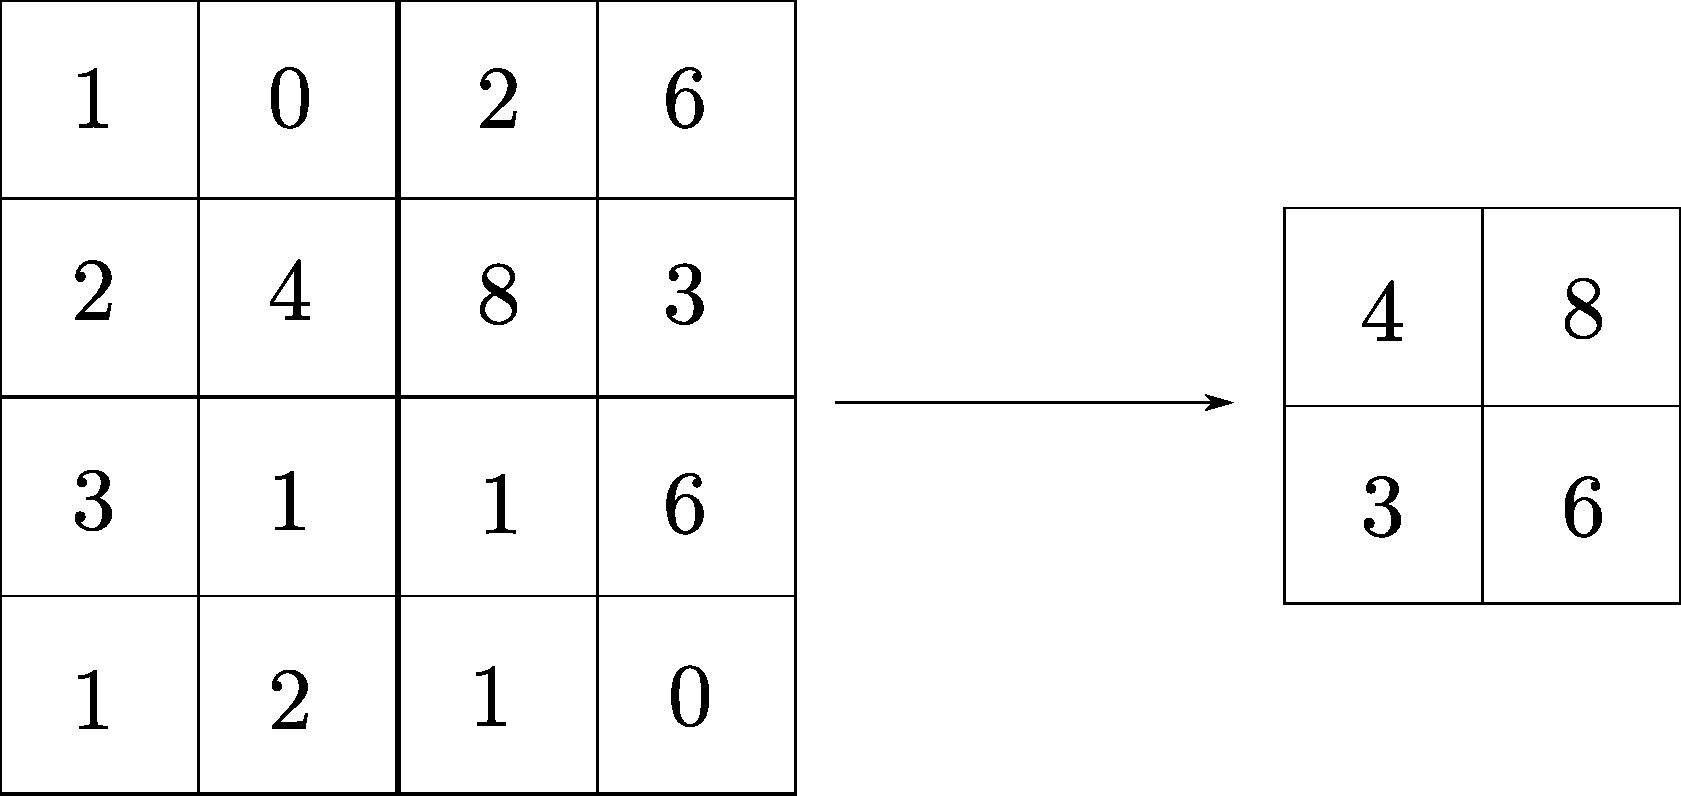
\includegraphics[scale=0.40]{max_pool.pdf}
	\caption{Sažimanje maksimalnom vrijednošću s filterom veličine 2x2 i korakom 2}
	\label{fig:max_pool}
\end{figure}
Ovaj sloj ne uvodi dodatne parametre u mrežu.

\section{Rezidualna neuronska mreža}
Duboke konvolucijske neuronske mreže su se pokazale jako učinkovite pri
rješavanju problema iz područja računalnog vida. Također se pokazalo da je
dubina neuronske mreže jako važna. Ali nakon određenog broja slojeva
dolazi do problema nestajućih i eksplodirajućih gradijenata što sprječava 
učenje od početka. Ovaj problem se u velikoj mjeri rješava normaliziranim
inicijaliziranjem i normalizacijskim slojevima, što omogućava mrežama s
desetak slojeva konvergirati. Međutim, pojavio se problem degradacije: 
kako se dubina mreže povećava točnost mreže počinje naglo opadati.
\\\indent Kao rješenje navedenog problema razvile su se rezidualne
neuronske mreže koje koriste rezidualne blokove definirane u 
\cite{DBLP:journals/corr/HeZRS15}. Ovi blokovi uvode nove
veze u slojevima zvane prečice koje preskaču jedan ili više slojeva i zbrajaju
se s izlazom zadnjeg preskočenog sloja. Kako se izlaz iz prečice zbraja sa
izlazom preskočenih slojeva dimenzije im se moraju podudarati.
\\\indent Rezidualni blokovi rješavaju problem degradacije, te dodavanjem
novih slojeva pospješuju se rezultati, ali se povećava broj parametara.
Za mreže s 50 slojeva i više koriste se rezidualni blokovi s uskim grlom, kako 
bi smanjili broj parametara. Kod običnih rezidualnih blokova koriste se
dva konvolucijska sloja s filterima veličine 3x3, dok blok s uskim grlom
koristi jednu takvu konvoluciju i dvije konvolucije s filterima veličine 1x1
ispred i iza nje. Prva konvolucija smanjiva broj filtera, dok zadnja 
povećava na početni broj kako bi se omogućilo zbrajanje s izlazom iz prečice.

\chapter{Implementacija}
Programska implementacija konvolucijskog modela za jednooku predikciju dubine 
scene ostvarena je po uzoru na rad \citep{DBLP:journals/corr/LainaRBTN16} uz
manje promjene.

\section{Korišteni alati i tehnologije}
Za izradu rada korišten je programski jezik Python\footnote{https://
www.python.org}, radno okruženje PyTorch\footnote{https://pytorch.org},
te biblioteke Numpy\footnote{https://www.numpy.org}, h5py\footnote{https://
www.h5py.org}, matplotlib\footnote{https://matplotlib.org}, sckit-image
\footnote{https://scikit-image.org/}. Biblioteka Numpy je korištena za efikasno 
izvršavanje različitih operacija nad matricama, dok je biblioteka sckit-image 
korištena za učitavanje slika. 
Biblioteka h5py korištena je za jednostavno spremanje i učitavanje slika.
Za vizualizaciju podataka i rezultata korištena je biblioteka matplotlib.
\\\indent Veći dio programske implementacije napisan je koristeći radno
okruženje PyTorch. Verzija PyTorcha u kojoj je pisana programska implementacija
je 1.0.1. Jedna od bitnijih karakteristika ovog radnog okruženja je njegov
tensor koji je jako sličan Numpy-ovom polju s dodatkom da se
može izvoditi na GPU koji podržava CUDA što omogućava veću brzinu izvođenja.
Još jedno bitno svojstvo PyTorcha je to što omogućava jednostavnu implementaciju
propagacije pogreške unatrag. Prilikom izvršavanja matematičkih operacija 
nad tensorima PyTorch sprema koje su se operacije izvodile i pomoću toga
izračunava gradijente. Ova metoda zove se automatska diferencijacija i 
implementirana je u modulu \textit{Autograd}.
\\\indent Jednostavan primjer automatske diferencijacije u PyTorchu:
\begin{lstlisting}[numbers=left, language=Python, frame=single]
import torch

x = torch.ones(1, requires_grad=True) #tensor([1.])
y = x + 2 #tensor([3.])
z = y * y * 3 #tensor([27.])

z.backward() #racunanje gradijenata unatrag

print(x.grad) #dz/dx = 18 

\end{lstlisting}

\section{NYU Depth podaci}
Neuronska mreža je trenirana na \textit{NYU Depth v2} skupu podataka.
Skup se sastoji od slijeda videa iz raznih scena iz zatvorenih prostora 
koje su snimane s RGB i dubinskom kamerom Microsoft Kinect. Ukupno ima
464	scene iz 3 različita grada, 1449 gusto označenih usklađenih parova
RGB slika i dubinskih slika, te 407024 neusklađenih slika. Označeni podatci
su prethodno obrađeni da popune nedostajuće dubinske oznake, dok su ostali
podatci neobrađeni.
\begin{figure}[htb]
	\centering
	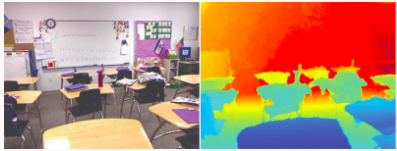
\includegraphics[scale=1]{labeled.png}
	\caption{Primjer prethodno obrađenih podataka}
	\label{fig:lab}
\end{figure}
\begin{figure}[htb]
	\centering
	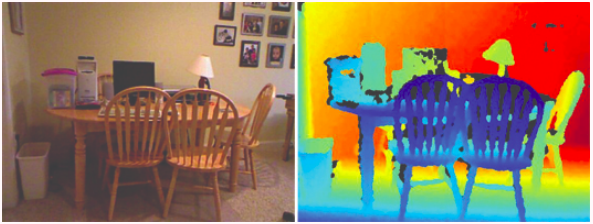
\includegraphics[scale=0.7]{raw.png}
	\caption{Primjer neobrađenih podataka}
	\label{fig:lab}
\end{figure}
\newpage  
\section{Priprema podataka}
Treniranje neuronske mreže se provodi nadziranim učenjem nad neobrađenim 
podatcima. Neobrađeni podatci se sastoje od 464 scene s podjelom na 249
scene za treniranje i 215 za testiranje. Za treniranje se međutim koristi 
mali podskup slika iz 242 scene za treniranje. Iz svake scene uzorkovano je 
50 jednako udaljenih slika i odgovarajućih dubinskih slika, što je rezultiralo
od ukupno 12100 parova RGB-D slika. Prilikom treniranja provodi se umjetno
proširivanje skupa za učenje čime se dobiva blizu 95000 RGB-D parova.
\\\indent Ulazne RGB slike imaju dimenzije 640x480, te se moraju svesti na 
dimenzije ulaza u neuronsku mrežu. Prvo se uzorkuju (engl. \textit{down-sample})
na pola veličine, zatim se odrežu u sredini na dimenzije 304x228.
\\\indent Nad tim ulaznim RGB slikama se primjenjuju transformacija za
umjetno proširivanje skupa podataka. Transformacije koje se primjenjuju:
\begin{itemize}
	\item Skaliranje: ulazne slike i dubinske mape se skaliraju sa 
	$s \in [1, 1.5]$ i dubinske mape se dijele sa $s$.
	\item Rotacija: ulazne slike i dubinske mape se rotiriaju za 
	$r \in [-5, 5]$ stupnjeva.
	\item Translacija: ulazne slike i dubinske mape su odrezane na
	nasumično odabranim mjestima kako bi im dimenzije odgovarale 
	dimenzijama ulaza u mrežu.
	\item Boja: ulazne slike se množe s nasumičnom RGB vrijednosti
	$c \in [0.8, 1.2]^3	$.
	\item Okretanje: ulazne slike i dubinske mape su vodoravno preokrenute
	s vjerojatnošću od 0.5.
\end{itemize}
Ovaj postupak se ponavlja 8 puta za svaki RGB-D par.

\section{Arhitektura modela}
Arhitektura neuronske mreže se nadograđuje na ResNet-50 model. Zamjenjuje se
zadnji potpuno povezani sloj, koji je dio izvorne arhitekture, s novim blokovima
za naduzorkovanje, čime se dobiva izlaz koji približno duplo manje 
dimenzije od ulaza. Zadnji konvolucijski sloj ResNet-50 modela proizvodi 
izlaz s 2048 mapi značajki s dimenzijama 10x8, zatim se blokovima za 
naduzorkovanje postiže izlaz dimenzija 160x128 piksela. Arhitektura 
modela je vidljiva na slici \ref{fig:model}.
\begin{figure}[htb]
	\centering
	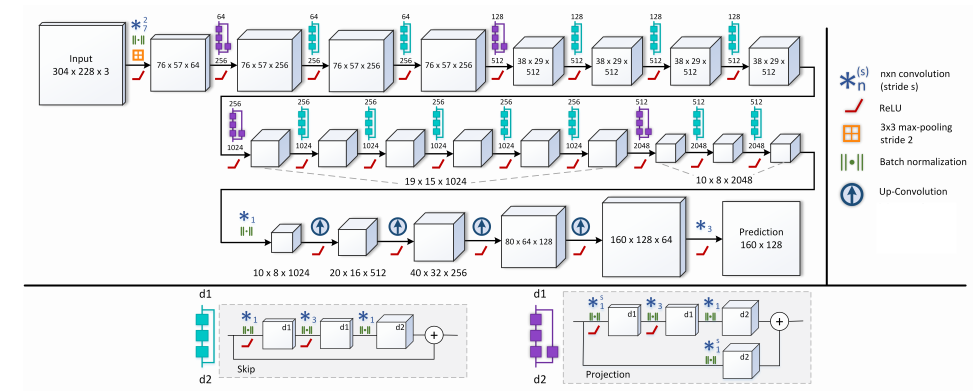
\includegraphics[scale=0.45]{model.png}
	\caption{Arhitektura modela}
	\label{fig:model}
\end{figure}

\indent Kako bi se povećala rezolucija izlaza uvode se novi blokovi za
naduzorkovanja zvano up-convolution blokovi. Cilj ovih blokova je
povećati za duplo dimenzije ulaza, tako da preslikavaju svaki ulaz
u gornji lijevi kut filtera veličine 2x2, a ostatak filtera se puni nulama. 
Nakon svakog takvog sloja slijedi konvolucijski sloj s filterom veličine 5x5 i 
zatim ReLU sloj. Up-convolution blok vidljiv je na slici \ref{fig:upconv}.

\begin{figure}[htb]
	\centering
	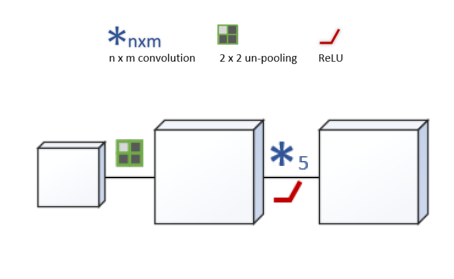
\includegraphics[scale=0.45]{up-conv.png}
	\caption{Up-convolution blok}
	\label{fig:upconv}
\end{figure}

Ovaj blok se dalje proširuje kako bi se stvorio up-projection blok. Nakon
up-convolution bloka dodaje se 3x3 konvolucija i rezultatu se dodaje
projekcijska veza iz mape značajki s manjom rezolucijom kako je prikazano na 
slici \ref{fig:upproj}. Zbog razlike u dimenzijama, manje mape značajki trebaju
se naduzorkovati s još jednim up-convolution blokom. Prva operacija 
up-convolution bloka se primjenjuje za obje grane zajedno, a zatim se 5x5
konvolucija primjenjuje odvojeno.
\begin{figure}[htb]
	\centering
	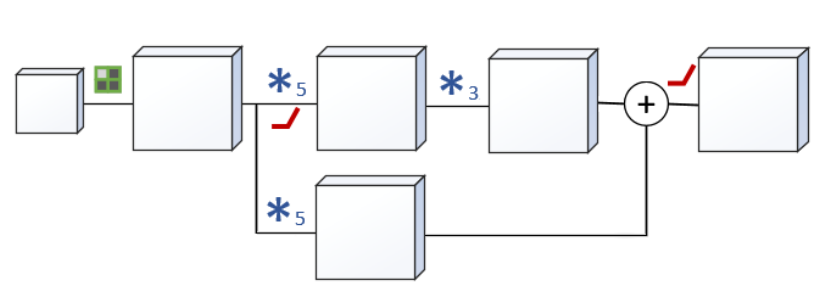
\includegraphics[scale=0.45]{up-proj.png}
	\caption{Up-projection blok}
	\label{fig:upproj}
\end{figure}

Kako bi se povećala učinkovitost up-convolution bloka uvodi se novi
brzi up-convolution blok. Nakon primjene prve operacije u up-convolution
bloku $75\%$ brojeva u izlaznim mapama značajki su nule, prema tome 5x5
konvolucija većinom djeluje na nulama, što se može izbjeći. Ovo se može
vidjeti na slici \ref{fig:fast}.

\begin{figure}[htb]
	\centering
	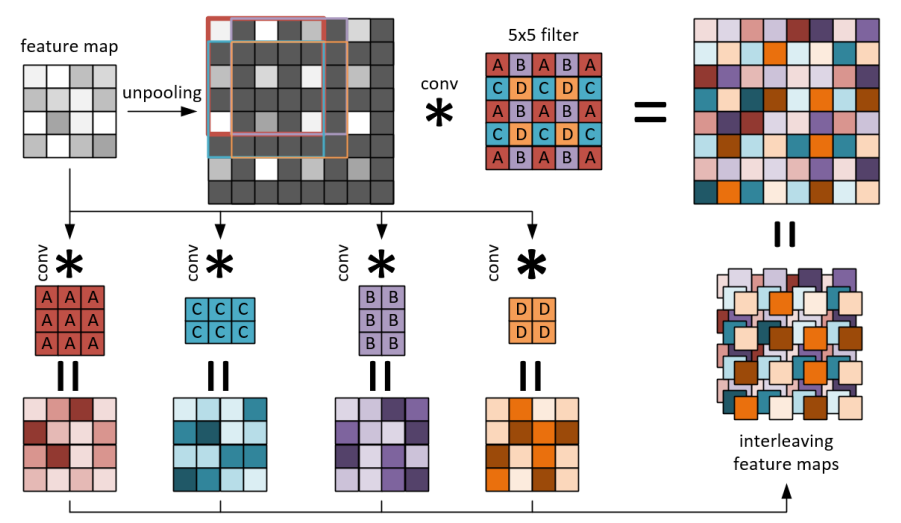
\includegraphics[scale=0.45]{fast.png}
	\caption{Način rada brzog up-convolution bloka}
	\label{fig:fast}
\end{figure}
Nakon povećavanja dimenzije mapi značajki, te primjene 5x5 konvolucije, samo
se određene težine množe s vrijednostima koje nisu nula. Te težine se dijele
na četiri grupe koje se ne preklapaju, prikazane oznakama A,B,C,D i različitim
bojama. Na temelju te četiri grupe izvorna 5x5 konvolucija se zamjenjuje s četiri nova
filtera dimenzija 3x3 (A), 3x2 (B), 2x3 (C), 2x2 (D). Isti izlaz se sad može 
ostvariti kao i kod izvornih operacija umetanjem elemenata iz četiri nove
mape značajki kao što je prikazano na slici \ref{fig:fast}. Brzi
up-convolution blok koji koristi ovu metodu prikazan je na slici \ref{fig:fastc}.

\begin{figure}[htb]
	\centering
	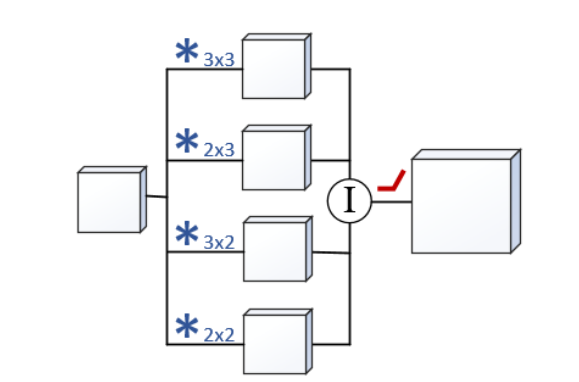
\includegraphics[scale=0.45]{fast-conv.png}
	\caption{Brzi up-convolution blok}
	\label{fig:fastc}
\end{figure}
Kako se kod običnog up-convolution bloka uvodi novi up-projection blok, tako
se i za brzi up-convolution blok uvodi novi brzi up-projection blok. Njegova
arhitektura prikazana je na slici \ref{fig:fastp}.
\begin{figure}[htb]
	\centering
	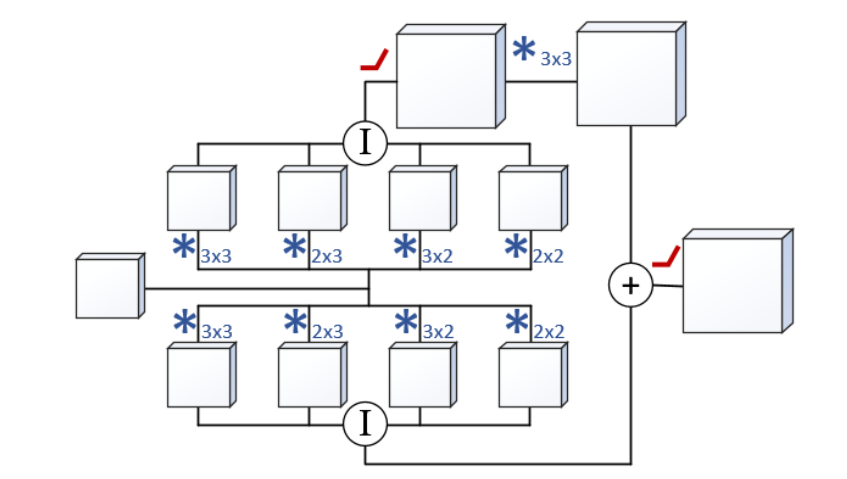
\includegraphics[scale=0.45]{fast-proj.png}
	\caption{Brzi up-projection blok}
	\label{fig:fastp}
\end{figure}

\chapter{Rezultati}

\chapter{Zaključak}
Zaključak.

\bibliography{literatura}
\bibliographystyle{fer}
\nocite{Cupic-UNN}
\nocite{Goodfellow-et-al-2016}
\nocite{DBLP:journals/corr/HeZRS15}


\begin{sazetak}
Sažetak na hrvatskom jeziku.

\kljucnerijeci{Ključne riječi, odvojene zarezima.}
\end{sazetak}

% TODO: Navedite naslov na engleskom jeziku.
\engtitle{Title}
\begin{abstract}
Abstract.

\keywords{Keywords.}
\end{abstract}

\end{document}
